%\documentclass[11pt]{article}
%\usepackage{graphicx}
%\RequirePackage{psfrag}
%\RequirePackage{fancyhdr}
%\RequirePackage{fancybox}
%\RequirePackage{fancyvrb}
%\RequirePackage{sectsty}
%\RequirePackage{amsmath}
%\RequirePackage{amssymb}
%\RequirePackage{makeidx}
%\usepackage{moreverb,relsize,ttname}
%\RequirePackage{url}
%\RequirePackage[latin1]{inputenc}
%\RequirePackage[colorlinks]{hyperref}

%\newcommand{\emp}[1]{{\smaller\texttt{#1}}}
%\DefineVerbatimEnvironment{code}{Verbatim}{frame=single,rulecolor=\color{blue},fontsize=\small}

\fenicschapter{Instant: Just-in-Time Compilation of C/C++ Code in Python}
              {Instant: Just-in-Time Compilation of C/C++ Code in Python}
              {Ilmar M. Wilbers, Kent-Andre Mardal and Martin S. Aln{\ae}s}
              {wilbers}

%\label{Instant}
%\begin{document}

%\maketitle
%\vspace{-0.3cm}

%\thispagestyle{empty}

\section{Introduction}

Instant is a small Python module for just-in-time compilation (or inlining) of
C/C++ code based on \index{SWIG}SWIG~\cite{www:swig} and
\index{Distutils}Distutils\footnote{http://www.python.org/doc/2.5.2/lib/module-distutils.html}. 
Just-in-time compilation can significantly speed up, e.g., your NumPy~\cite{www:numpy} code in a clean and
readable way. This makes Instant a very convenient tool in combination with code
generation. Before we demonstrate the use of Instant in a series of examples,
we briefly step through the basic ideas behind the implementation.
Instant relies on SWIG for the generation of wrapper code needed for making the
C/C++ code usable from Python~\cite{www:python}. SWIG is a mature and well-documented tool
for wrapping C/C++ code in many languages. We refer to its website for a comprehensive 
user manual and we also discuss some common tricks and troubles in Chapter~\ref{chap:mardal-2}. 
The code to be inlined, in addition to the
wrapper code, is then compiled into a Python extension module (a shared library
with functionality as specified by the Python C-API) by using
Distutils. To check whether the C/C++ code has changed since the last
execution, Instant computes the SHA1
sum\footnote{http://www.apps.ietf.org/rfc/rfc3174.html} of the code and compares it to
the SHA1 checksum of the code used in the previous execution. Finally, Instant has
implemented a set of SWIG \index{typemaps}typemaps, allowing the user to
transfer NumPy arrays between the Python code and the C/C++ code.

There exist several packages that are similar to Instant. 
Worth mentioning here are \index{Weave}Weave~\cite{www:weave}, 
\index{Cython}Cython~\cite{www:cython}, and \index{F2PY}F2PY~\cite{Peterson}. 
Weave allows us to inline C code directly in our Python
code. Unlike Instant, Weave does not require the specification of the function
signature and the return argument. For specific examples of Weave and the
other mentioned packages, we refer to~\cite{WilbersLangtangenEtAl2009,www:weave}. Weave is part of
SciPy~\cite{www:scipy}. 
%FIXME this needs to be put another place:
%Indexing multi-dimensional arrays in Instant and Weave must
%be done by using striding as the different dimensions are stored in
%consecutive order in a single, one-dimensional array. Hence, indexing the
%element $i,j,k$ in the three-dimensionsl array $u$ is done by writing $u[i*m +
%j*n + k]$ instead of the more natural $u(i,j,k)$. The latter syntax can be
%achieved with Weave by using Blitz++ arrays, at the cose of speed.
F2PY is currently part of NumPy, and is primarily intended
for wrapping Fortran code. F2PY can also be used for wrapping C
code. 
%FIXME: this needs to be put another place:
%By including special comment lines, we can specify how the arguments
%sent back and forth between Python and the Fortran code should be
%treated. Since Fortran using column-major storage, while Python (and C) use
%row-major storage, it is important to specify the storage of the NumPy arrays
%correctly in order to gain the maximum speed-up.
Cython is a rather new project, branched from the more well-known Pyrex
project~\cite{www:pyrex}. Cython is attractive because of  its integration
with NumPy arrays. Cython differs from the other projects by being a programming
language of its own. Cython extends Python with concepts such as static typing,  
hence allowing the user to incrementally speed up the code.

Instant accepts plain C/C++. This makes it particularly attractive to combine
Instant with tools capable of generating C/C++ code such as FFC (see Chapter~\ref{chap:logg-1}),
SFC (see Chapter~\ref{chap:alnes-3}), Swiginac~\cite{www:swiginac}, and Sympy~\cite{Certik2009}.  In fact,
tools like these have been the main motivation behind Instant, and both FFC
and SFC employ Instant. Instant is released under a BSD license, see the
file \emp{LICENSE} in the source directory.

In this chapter we will begin with several examples in Section \ref{wilbers:sec:examples}.  
Section \ref{wilbers:sec:explained} explains how Instant works, while 
Section \ref{wilbers:sec:api} gives a detailed description of the API. 


\section{Examples}
\label{wilbers:sec:examples}
All code from the examples in this section can be found
online\footnote{http://www.fenics.org/pub/documents/book/instant/examples}.
We will refer
to this location as \emp{\$examples}.

\subsection{Installing Instant}
Before trying to run the examples, you need to install Instant.
The latest Instant release can be downloaded from the FEniCS
website~\cite{www:fenics}. It is
available both as a source code tarball and as a Debian package. In addition, the latest
source code can be checked out using
Mercurial~\cite{www:mercurial}:
\begin{code}
hg clone http://www.fenics.org/hg/instant
\end{code}
Installing Instant
from the source code is done with a regular Distutils script, i.e,  
\begin{code}
python setup.py install
\end{code}
After successfully
installing Instant, one can verify the installation by running the scripts
\emp{run\_\-tests.py} followed by \emp{rerun\_\-tests.py} in the
\emp{tests}-directory of the source code. The first will run all the examples after having
cleaned the Instant cache, the second will run all examples using the
compiled modules found in the Instant cache from the previous execution. 
%If PyChecker\footnote{http://pychecker.sourceforge.net/} is installed, one can
%also run \emp{run\_\-pychecker.py}. 


\subsection{Hello World}
Our first example demonstrate the usage of Instant in a very simple case:
\begin{code}
from instant import inline
c_code = r'''
double add(double a, double b)
{
  printf("Hello world! C function add is being called...\n");
  return a+b;
}'''
add_func = inline(c_code)
sum = add_func(3, 4.5)
print 'The sum of 3 and 4.5 is', sum
\end{code}
Here Instant will wrap the C-function \emp{add} into a Python extension module by using
SWIG and Distutils. 
The inlined function is written in standard C. SWIG supports almost
all of C and C++, including object orientation and templates. When running
this Python snippet the first time, compiling the C code takes a few seconds. Next time we run
it, however, the compilation is omitted, given that no changes are made to the
C source code. 

Note that a raw string is used in this example, to avoid
Python interpreting escape sequences such as '\verb@\@\emp{n}'. Alternatively,
special characters can be escaped using a backslash.

Although Instant notifies the user when it is compiling, it might
sometimes be necessary, e.g. when debugging, to see the details of the Instant
internals. We can do this by setting the logging level before calling any
other Instant functions:
\begin{code}
from instant import output
output.set_logging_level('DEBUG')
\end{code} 
The intrinsic Python module \emp{logging} is used. First, the 
\emp{build\_\-function} arguments are displayed, whereafter the different steps
performed by Instant are shown in detail, e.g whether the module is found in
cache and the arguments to the Distutils file when building the module. 
This example can be found in the file \emp{\$examples/ex1.py}.


\subsection{NumPy Arrays}
One basic problem with wrapping C and C++ code is how to handle dynamically
allocated arrays. Arrays allocated
dynamically are typically represented in C/C++ by a pointer to the first element
of an array and a separate integer variable holding the array size. In Python
the array variable is itself an object contains the data array, array size, 
type information etc. However, a pointer in C/C++ does not necessarily
represent an array. Therefore, SWIG provides the typemap functionality 
that allows the user to specify a mapping between Python and C/C++ types. We
will not go into details on typemaps in this chapter, but the reader 
should be aware that it is a powerful tool that may greatly enhance your 
code, but also lead to mysterious bugs when used wrongly. Typemaps 
are discussed in Chapter~\ref{chap:mardal-2} and at length at the SWIG
webpage. In this chapter, it is sufficient to illustrate how to deal
with arrays in Instant using the NumPy module. More details on how Instant
NumPy arrays can be found in Section \ref{wilbers:sec:arrays}.

\subsection{Ordinary Differential Equations}
We introduce a
solver for an ordinary differential equation (ODE) modeling blood pressure by
using a \index{Windkessel model}Windkessel model. The ODE is as follows:
\begin{eqnarray}
\frac{d}{dt}p(t) &=& B Q(t) - A p(t), \quad t \in (0,1), \\ 
p(0) &=& p0.   
\end{eqnarray}
Here $p(t)$ is the blood pressure, $Q(t)$ is the volume flux of blood,  
$A$ is $\ldots$ and $B$ is $\ldots$.  
An explicit scheme is:
\begin{eqnarray}
p_i &=& p_{i-1} + \Delta t (B Q_i - A p_{i-1}), \quad \mbox{for}\quad i=1,\ldots,N-1,  \\ 
p_0 &=& p0.
\end{eqnarray}
The scheme can be implemented in Python as follows using NumPy arrays:
\begin{code}
def time_loop_py(p, Q, A, B, dt, N, p0): 
    p[0] = p0 
    for i in range(1, N): 
        p[i] = p[i-1] + dt*(B*Q[i] - A*p[i-1])
\end{code}
The C code given as argument to the Instant function \emp{inline\_\-with\_\-numpy}
looks like:
\begin{code}
void time_loop_c(int n, double* p,
                 int m, double* Q,
                 double A, double B,
                 double dt, int N, double p0)
{
    if ( n != m || N != m )
    {
        printf("n, m and N should be equal\n");
        return;
    }

    p[0] = p0;
    for (int i=1; i<n; i++)
    {
        p[i] = p[i-1] + dt*(B*Q[i] - A*p[i-1]);
    }
}
\end{code}
In this example, \emp{(int n, double* p)} represents an array of doubles with
length $n$. However, this can not be determined by the function signature:
\begin{code}
void time_loop_C(int n, double* p, int m, double* Q, ...) 
\end{code}
For example, \emp{double* p} may be an array of length $m$ or it may simply be
output. In Instant
you can specify 1-dimensional arrays as follows:
\begin{code}
time_loop_c = inline_with_numpy(c_code,
                                arrays = [['n', 'p'],
                                          ['m', 'Q']])
\end{code}
Here we tell Instant that \emp{(int n, double* p)} and  
\emp{(int m, double* Q)} are NumPy arrays (and Instant then employs
a few typemaps). 
We may then call the \emp{time\_\-loop}
function as follows: 
\begin{code}
time_loop_c(p, Q, 1.0, 1.0, 1.0/(N-1), N, 1.0)
\end{code}
In the above example we obtain a speed-up of about a factor 400 when using
100000 time steps compared to the pure Python with NumPy version, see Table
\ref{wilbers:fig:speed-up}. This is about the same as a pure C program. The result of
solving the ODE can be seen in Figure
\ref{wilbers:fig:fig1}. The comparison between NumPy and Instant is not really fair, as
NumPy  primarily gives a speed-up for code that can be vectorized, something
that is not the case with our current ODE. In fact, utilizing pure Python
lists instead of NumPy arrays, reduces the speed-up to a factor 100. For code
that can be vectorized, the speed-up is about one order of magnitude when we
use Instant instead~\cite{WilbersLangtangenEtAl2009}.

\begin{figure}
\begin{center}
\includegraphics[width=100mm]{chapters/wilbers/eps/pressure_plot.eps}
\caption{Plot of pressure and blood volume flux computed by solving the Windkessel model.}
\label{wilbers:fig:fig1}
\end{center}
\end{figure}

\begin{table}[h]
\begin{center}
\begin{tabular}{|l|c|c|c|c|c|} \hline
N                     & 100     & 1000   & 10000  & 100000 & 1000000 \\ \hline 
CPU time with NumPy   & 3.9e-4  & 3.9e-3 & 3.8e-2 & 3.8e-1 & 3.8     \\ \hline 
CPU time with Python  & 0.7e-4  & 0.7e-3 & 0.7e-2 & 0.7e-1 & 0.7     \\ \hline 
CPU time with Instant & 5.0e-6  & 1.4e-5 & 1.0e-4 & 1.0e-3 & 1.1e-2  \\ \hline
CPU time with C       & 4.0e-6  & 1.1e-5 & 1.0e-4 & 1.0e-3 & 1.1e-2  \\ \hline 
\end{tabular}
\caption{CPU times of Windkessel model for different implementations (in seconds).}
\label{wilbers:fig:speed-up}
\end{center}
\end{table}
The complete code for this example can be found in \emp{\$examples/ex2.py}


\subsection{Numpy Arrays and OpenMP}
It is easy to speed up code on parallel computers with OpenMP. We will not
describe \index{OpenMP}OpenMP in 
any detail here, the reader is referred to~\cite{www:openmP}. However, note
that preprocessor directives like '\emp{\#pragma omp \ldots}' are OpenMP directives and
that OpenMP functions start with \emp{omp}.
In this example, we want
to solve a standard 2-dimensional wave equation in a heterogeneous medium with
local wave velocity $k$:
\begin{equation}
\frac{\partial^2u}{\partial t^2} = \nabla \cdot [k\nabla u]\, .
\end{equation}
We set the boundary condition to $u = 0$ for the whole boundary of a
rectangular domain $\Omega = (0,1) \times (0,1)$. Further, $u$ has the initial
value $I(x,y)$ at $t = 0$ while $\partial u/ \partial t = 0$.
We solve the wave equation using the following finite difference scheme:
\begin{align}
u_{i,j}^l = 
&\left(\frac{\Delta t}{\Delta x}\right)^2
[k_{i+\frac{1}{2},j}(u_{i+1,j} - u_{i,j}) - k_{i-\frac{1}{2},j}(u_{i,j} - u_{i-1,j})]^{l-1}\notag\\
+&\left(\frac{\Delta t}{\Delta y}\right)^2
[k_{i,j+\frac{1}{2}}(u_{i,j+1} - u_{i,j}) - k_{i,j-\frac{1}{2}}(u_{i,j} - u_{i,j-1})]^{l-1}.
\end{align}\label{u}
Here, $u_{i,j}^l$ represents $u$ at the grid point $x_i$ and $y_j$ at
time level $t_l$, where
\begin{align*}
x_i &= i\Delta x, i = 0, \ldots, n\\
y_i &= j\Delta y, j = 0, \ldots, m\textrm{ and}\\
t_l &= l\Delta t,
\end{align*}
Also, $k_{i+\frac{1}{2},j}$ is short for $k(x_{i+\frac{1}{2}},y_j)$.

The code for calculating the next time step using OpenMP looks like:
\begin{code}
void stencil(double dt, double dx, double dy,
             int ux, int uy, double* u,
             int umx, int umy, double* um,
             int kx, int ky, double* k,
             int upn, double* up){
#define index(u, i, j) u[(i)*m + (j)]
  int i=0, j=0, m = ux, n = uy;
  double hx, hy, k_c, k_ip, k_im, k_jp, k_jm;
  hx = pow(dt/dx, 2); 
  hy = pow(dt/dy, 2);
  j = 0;   for (i=0; i<m; i++) index(up, i, j) = 0;
  j = n-1; for (i=0; i<m; i++) index(up, i, j) = 0;
  i = 0;   for (j=0; j<n; j++) index(up, i, j) = 0;
  i = m-1; for (j=0; j<n; j++) index(up, i, j) = 0;
  #pragma omp for
  for (i=1; i<m-1; i++){
    for (j=1; j<n-1; j++){
      k_c = index(k, i, j);
      k_ip = 0.5*(k_c + index(k, i+1, j));
      k_im = 0.5*(k_c + index(k, i-1, j));
      k_jp = 0.5*(k_c + index(k, i, j+1));
      k_jm = 0.5*(k_c + index(k, i, j-1));
      index(up, i, j) = 2*index(u, i, j) - index(um, i, j) + 
        hx*(k_ip*(index(u, i+1, j) - index(u, i, j)) - 
             k_im*(index(u, i, j) - index(u, i-1, j))) + 
        hy*(k_jp*(index(u, i, j+1) - index(u, i, j)) - 
            k_jm*(index(u, i, j) - index(u, i, j-1)));
    }
  }
}
\end{code}
We also need to add the OpenMP header \emp{omp.h} and compile
with the flag \emp{-fopenmp} and link with the OpenMP shared 
library, e.g. \emp{libgomp.so} for Linux (specified with \emp{-lgomp}). 
This can be done as follows:
\begin{code}
instant_ext = \
  build_module(code=c_code, 
               system_headers=['numpy/arrayobject.h', 
                               'omp.h'],
               include_dirs=[numpy.get_include()],
               init_code='import_array();',
               cppargs=['-fopenmp'], 
               lddargs=['-lgomp'],
               arrays=[['ux', 'uy', 'u'], 
               ['umx', 'umy', 'um'],
               ['kx', 'ky', 'k'],
               ['upn', 'up', 'out']])
\end{code}
Note that the arguments \emp{include\_\-headers}, \emp{init\_\-code}, and the
first element of \emp{system\_\-headers} could have been omitted had we chosen
to use \emp{inline\_\-module\_\-with\_\-numpy} instead of \emp{build\_\-module}. We could also
have used \emp{inline\_\-with\_\-numpy}, which would have returned only the
function, not the whole module. For more details, see the next section.
The complete code can be found in \emp{\$examples/ex3.py}. It might very well
be possible to write more efficient code for many of these examples, but the
primary objective is to examplify different Instant features.

%In Table \ref{speed-up2} we have compared the timings of running with
%different numbers of CPUs. The timings in this table are performed on a
%quad-core machine with 32GB memory. We see a speed-up of factor two when doubling the
%number of CPUs, but further increasing the number of CPUs has a limited
%effect. We have not been able to investigate this further, but suspect that
%he physical layout of the machine with two dual cores causes this, as the two
%PUs on the same core share some of the resources.
%\begin{table}[h]
%\begin{center}
%\begin{tabular}{|l|c|c|} \hline
%N                     & 1e+8     &2e+8 \\ \hline 
%CPU time with Instant 1 CPU & 0.80  & 1.59  \\ \hline 
%CPU time with Instant 2 CPU & 0.42  & 0.81  \\ \hline 
%CPU time with Instant 3 CPU & 0.37  & 0.75  \\ \hline 
%CPU time with Instant 4 CPU & 0.34  & 0.67  \\ \hline 
%\end{tabular}
%\caption{CPU times for Instant with OpenMP (in seconds).}
%label{speed-up2}
%end{center}
%end{table}

%\subsection{Code Generation}
%Instant is often used together with code generation tools (or compilers) such
%as FFC~\cite{FFC} and SFC~\cite{SFC}. While these compilers are advanced
%tools that translate abstract formulations of finite element methods into C++,
%Instant has a relatively simple role in this picture. We will illustrate this
%here in a simple situation. We will assume that we want to solve the Poisson
%equation
%\begin{equation}
%-\Delta u = f,   
%\end{equation}
%and that we want to use the so-called 'method of manufactured solution' to check the
%convergence of the error as a function of the mesh size parameter $h$. This method 
%include the following steps: 
%\begin{enumerate}
%\item find an analytical expression for $u$, 
%\item compute $f=-\Delta u$, 
%\item solve the Poisson equation using the source
%term $f$ and Dirichlet boundary conditions set as $u$ on the whole boundary, 
%\item compute the difference between the analytical solution $u$ and the computed
%solution $u_h$, as a function of $h$. 
%\end{enumerate}
%The following code, found in \emp{\$examples/ex7.py}, shows how  
%we can compute the source term $f$ as a function of the analytical solution
%$u$, using \index{Swiginac}Swiginac~\cite{Swiginac}
%\begin{code}
%from swiginac import *
%x = symbol('x'); y = symbol('y')
%u = sin(x*x)*cos(y); 
%f = - diff(diff(u,x),x) - diff(diff(u,y),y)
%\end{code}
%In the following we generate code for a Dolfin \emp{Function}
%\begin{code}
%def expression2string(name, expression):
%    c_code = """
%    #include <dolfin.h>
%    using namespace dolfin;
%    class %s : public Function 
%    {
%        virtual double eval(const double* p) { 
%            const double x = p[0];  
%            const double y = p[1];  
%            return %s; 
%        }
%    };
%    """ % expression.printc()
%    return (name, c_code)
%\end{code}
%Finally, we inline this Dolfin function using Instant as follows
%\begin{code}
%(includes, flags, libraries, libdirs) = \ 
%            instant.header_and_libs_from_pkgconfig("dolfin")
%U_module = instant.inline_module(expression2string("u", u), \
%         system_headers=includes, cppargs=flags, lddargs=libraries,\
%         library_dirs=libdirs) 
%U = U_module.U
%F_module = instant.inline_module(expression2string("f", f), \
%         system_headers=includes, cppargs=flags, lddargs=libraries,\ 
%         library_dirs=libdirs) 
%F = F_module.F
%
%\end{code}
%
%Since, \emp{U} and \emp{F} are now standard Dolfin functions they can be used 
%in a standard fashion and solving the Poisson equation is then done as follows
%\begin{code}
%# Define boundary condition
%bc = DirichletBC(V, U, DirichletBoundary())
%
%# Define variational problem
%v = TestFunction(V)
%u = TrialFunction(V)
%a = inner(grad(v), grad(u))*dx
%L = v*F*dx
%
%# Compute solution
%problem = VariationalProblem(a, L, bc)
%u = problem.solve()
%\end{code}
%The complete code is found in \emp{\$examples/ex8.py}).
%
%Notice that Instant is also used in assembly here, where either FFC or SFC translate the UFL
%description of the variational problem into (UFC-compliant) C++ code that is inlined with 
%Instant. We refer to the Chapters~\ref{FFC},~\ref{SFC},~\ref{UFC},
%and~\ref{UFL} for more information on this.   
%We also remark that Dolfin has functionality for compiling functions and that the above
%code is only meant for illustration. The reader is encouraged to use this functionality instead
%of the more manual approach described above. It is done as follows:     
%\begin{code}
%# Source term, using compiled C++ expression
%class Source(Function):
%    cppexpr = ("A*exp(-(pow(x[0]-0.5,2) + pow(x[1]-0.5,2))/B)")
%    default = {"A":500.0,"B":0.02}
%\end{code}
%Code generation example (advanced with SFC). FIXME: Martin should we give more details
%about how instant can be used more generally here ? .
%

\section{Instant Explained}
\label{wilbers:sec:explained}

The previous section concentrated on the usage of Instant and it may
appear mysterious how it actually works since it is unclear what
files that are made during execution and where they are located. 
In this section we explain this. 

We will again use our first example, but this time with
the keyword argument \emp{modulename} set explicitely. The file can be found
under \emp{\$examples/ex4.py}:
\begin{code}
from instant import inline
code = r'''
double add(double a, double b)
{
  printf("Hello world! C function add is being called...\n"); 
  return a+b;
}'''
add_func = inline(code, modulename='ex4_cache') 
sum = add_func(3, 4.5)
print 'The sum of 3 and 4.5 is', sum
\end{code}
Upon calling Instant the first time for some C/C++ code, Instant compiles this
code and stores the resulting files in a directory \emp{ex4\_\-cache}. The
output from running the code the first time is:
\begin{code}
--- Instant: compiling ---
Hello world! C function add is being called...
The sum of 3 and 4.5 is 7.5
\end{code}
Next time we ask
Instant to call this code, it will check if the compiled files are available
either in cache or locally, and further whether we need to rebuild these files
based on the checksum of the source files and the arguments to the Instant
function. This means that Instant will perform the compile step \emph{only} if
changes are made to the source code or arguments. More details about the
different caching options can be found in Section \ref{wilbers:sec:msc}. 

The resulting module files can be found in a directory reflecting the name of
the module, in this case \emp{ex4\_\-cache}:
\footnotesize
\begin{code}
ilmarw@multiboot:~/instant_doc/code$ cd ex4_cache/
ilmarw@multiboot:~/instant_doc/code/ex4_cache$ ls -g
total 224
drwxr-xr-x 4 ilmarw  4096 2009-05-18 16:52 build
-rw-r--r-- 1 ilmarw   844 2009-05-18 16:52 compile.log
-rw-r--r-- 1 ilmarw   183 2009-05-18 16:52 ex4_cache-0.0.0.egg-info
-rw-r--r-- 1 ilmarw    40 2009-05-18 16:52 ex4_cache.checksum
-rw-r--r-- 1 ilmarw   402 2009-05-18 16:53 ex4_cache.i
-rw-r--r-- 1 ilmarw  1866 2009-05-18 16:52 ex4_cache.py
-rw-r--r-- 1 ilmarw  2669 2009-05-18 16:52 ex4_cache.pyc
-rwxr-xr-x 1 ilmarw 82066 2009-05-18 16:52 _ex4_cache.so
-rw-r--r-- 1 ilmarw 94700 2009-05-18 16:52 ex4_cache_wrap.cxx
-rw-r--r-- 1 ilmarw    23 2009-05-18 16:53 __init__.py
-rw-r--r-- 1 ilmarw   448 2009-05-18 16:53 setup.py
\end{code}
\normalsize
When building a new module, Instant creates a new directory with 
a number of files. The first file it generates is the SWIG interface file, named
\emp{ex4\_\-cache.i} in this example. Then the Distutils file \emp{setup.py} is generated based
and executed. During execution, \emp{setup.py} first runs SWIG in the interface file, 
producing \emp{ex4\_\-cache\_\-wrap.cxx} and \emp{ex4\_\-cache.py}. The first file
is then compiled into a shared library  \emp{\_\-ex4\_\-cache.so}
(note the leading underscore). A file \\\emp{ex4\_\-cache-0.0.0.egg-info}
and a directory \emp{build} will also be present as a result of these
steps. The output from executing the Distutils file is stored in the file
\emp{compile.log}.  Finally, a checksum file named
\emp{ex4\_\-cache.checksum} is generated, containing a checksum based on
the files present in the directory. The final step consists of moving the whole
directory from its temporary location to either cache or a user-specified
directory. The \emp{\_\-\_\-init\_\-\_\-.py} imports the module \emp{ex4\_\-cache}. 


The script \index{\emp{instant-clean}}\emp{instant-clean} removes
compiled modules from the Instant cache, located in the directory
\emp{.instant} in the home directory of the user running it. In addition, all
Instant modules located in the temporary directory where they were first
generated and compiled. It does not clean modules located elsewhere.

The script \index{\emp{instant-showcache}}\emp{instant-showcache} allow you to see the modules currently located in the
Instant cache:
\begin{code}
Found 1 modules in Instant cache:
test_cache
Found 1 lock files in Instant cache:
test_cache.lock
\end{code}
Arguments to this script will output the files matching the specified pattern,
for example will \emp{instant-showcache 'test*.i'} show the content of the
SWIG interface file for any module beginning with the letters \emp{test}.

\subsection{Arrays and Typemaps}\label{wilbers:sec:arrays}
Instant has support for converting NumPy arrays to C arrays and vice
versa. For arrays with up to three dimensions, the SWIG interface file from
NumPy is used, with a few modifications. When installing Instant, this file is
included as well. \emp{arrays} should be a list, each entry containing
information about a specific array. This entry should contain a list with
strings, so the \emp{arrays} argument is a nested list.\index{typemaps}

Each array (i.e. each element in \emp{arrays}) is a list containing the names
of the variables describing that array in the C code. For a 1-dimensional
array, this means the names of the variables containing the length of the
array (an \emp{int}), and the array pointer (can have several tpes, but the
default is \emp{double}). For 2-dimensional arrays we need three strings, two
for the length in each dimension, and the third for the array pointer. For
3-dimensional arrays, there will be three variables first. This example should
make things clearer
\begin{code}
arrays = [['len', 'a'],
          ['len_bx', 'len_by', 'b'],
          ['len_cx', 'len_cy', 'len_cz', 'c']]
\end{code}
These variables names specified reflect the variable names in the C function
signature. It is important that the order of the variables in the signature is
retained for each array, e.g. one cannot write:
\begin{code}
c_code = """
double sum (int len_a, int len_bx, int len_by,
            double* a, double* b)
{
  ...
}
"""
\end{code}
The correct code would be:
\begin{code}
c_code = """
double sum (int len_a, double* a,
            int len_bx,
            int len_by, double* b)
{
  ...
}
"""
\end{code}
The order of the arrays can be changed, as long as the arguments in the Python
function are changed as well accordingly.

\subsubsection{Data Types}
Default, all arrays are assumed to be of type \emp{double}, but several other
types are supported. These
are \emp{float}, \emp{short}, \emp{int}, \emp{long}, \emp{long
long}, \emp{unsigned short}, \emp{unsigned int}, \emp{unsigned long},
and \emp{unsigned long long}. The type can be specified by adding an
additional element to the list describing the array, e.g.
\begin{code}
arrays = [['len', 'a', 'long']]
\end{code}
It is important that there is correspondance between the type of the NumPy
array and the type in the signature of the C function. For arrays that are
changed in-place, the types have to match exactly. For arrays that are input or
output (see next section), one has to make sure that the implicit casting is done to a type with
higher accuracy. For input arrays, the C type must be of higher (or the
same) accuracy than the NumPy array, while for output arrays the NumPy array
type must be of higher (or the same) accuracy than the C array. The NumPy
type \emp{float32} corresponds to the C type \emp{float}, while \emp{float64}
corresponds to \emp{double}. The NumPy type \emp{float} is the same
as \emp{float64}. For integer arrays, the mapping
between NumPy types and C types depends on your system. Using \emp{long} as
the C type will work in most cases.

\subsubsection{Input/Output Arrays}
All arrays are assumed to be both input and output arrays, i.e. any changes to
arrays in the C code result in the NumPy array being changed in-place. For
performace purposes, this is desirable, as we avoid unecessary copying of
data. The NumPy SWIG interface file has support for both input and output
arrays in addition to changing arrays in-place. Input arrays do not need to be
NumPy arrays, but can be any type of sequence, e.g. lists and tuples. The
default behaviour of the NumPy SWIG interface file is to create new objects
for sequences that are not NumPy arrays, while using mere pointers to the data
of NumPy arrays. Instant deviates from this behaviour by taking copies of all
input data, allowing for the modification of the array in the C code, as might
be necessary for certain applications, while retaining the array as seen from
the Python code. An array is marked as input only by adding the additional element \emp{'in'}
to the list describing the array:
\begin{code}
arrays = [['len', 'a', 'in']]
\end{code}

It is also possible to create output arrays in the C code. Instead of creating
an array in the Python code and sending it as an in-place array to the C
code, the array is created by the wrapper code and returned. If there are are
multiple output arrays or the C function has a return argument, the wrapper
function returns a tuple with the different arguments. This approach is more
Python-like than changing arrays in-place. 

We only need to specify the length of the array when calling the wrapper
function. The limitation is that only 1-dimensional arrays are supported,
which means that we need to set the shape of the array manually after calling
the wrapper function. In the C code all arrays are treated as 1-dimensional,
so this does not affect the C code. An array is marked as input only by adding
the additional element \emp{'out'} to the list describing the array. The
following code shows an example where we calculate matrix-vector
multiplication $x = Ab$. The matrix $A$ is marked as input, the vector $b$ as
in-place, and the vector $x$ as output. The example is only meant for
illustrating the use of the different array options, and can be found in the
file \emp{\$examples/ex5.py}. We verify that the result is correct by using
the dot product from NumPy:
\begin{code}
from instant import inline_with_numpy
from numpy import arange, dot

c_code = '''
void dot_c(int Am, int An, long* A, int bn, int* b,
           int xn, double* x)
{
  for (int i=0; i<Am; i++)
  {
    x[i] = 0;
    for (int j=0; j<An; j++)
    {
      x[i] += A[i*Am + j]*b[j];
    }
  }
}
'''
dot_c = \
  inline_with_numpy(c_code,
                    arrays = [['Am', 'An', 'A', 'in', 'long'],
                              ['bn', 'b', 'int'],
                              ['xn', 'x', 'out']])
a = arange(9)
a.shape = (3, 3)
b = arange(3)

c1 = dot_c(a, b, a.shape[1])
c2 = dot(a, b)
print c1
print c2
\end{code}


\subsubsection{Multi-dimensional Arrays}
If one needs to work with arrays that are more than 3-dimensional, this is
possible. However, the typemaps used for this employ less error checking, and
can only be used for the C type \emp{double}. The list describing the array
should contain the variable name for holding the number of dimensions, the
variable name for an integer arrays holding the size in each dimension, the
variable name for the array, and the argument \emp{'multi'}, indicating that
it has more than 3 dimensions. The \emp{arrays} argument could for example be:
\begin{code}
arrays = [['m', 'mp', 'ar1', 'multi'],
          ['n', 'np', 'ar2', 'multi']]
\end{code}
In this case, the C function signature should look like:
\begin{code}
void sum (int m, int* mp, double* ar1, int n,
          int* np, double* ar2)
\end{code}

In the C code, all arrays are 1-dimensional. Indexing a 3-dimensional arrays
becames rather complicated because of striding. For instance, instead of
writing \emp{u(i,j,k)} we need to write \emp{u[i*ny*nz + j*ny + k]},
where \emp{nx}, \emp{ny}, and \emp{nz} are the lengths of the array in each
direction. One way of achieving a simpler syntax is to use the \emp{\#define}
macro in C:
\begin{code}
#define index(u, i, j, k) u[(i)*nz*ny + (j)*ny + (k)]
\end{code}
which allows us to write \emp{index(u, i, j, k)} instead.

\subsection{Module name, signature, and cache}\label{wilbers:sec:msc}
\index{cache}\index{signatures}
The Instant cache resides in the directory \emp{.instant} in the
directory of the user. It is possible to specify a different directory, but the
\emp{instant-clean} script will not remove these when executed.
The three keyword arguments \emp{modulename}, \emp{signature}, and
\emp{cache\_\-dir} are connected. If none of them are given, the default behaviour is to
create a signature from the contents of the files and arguments to the
\emp{build\_\-module} function, resulting in a name starting with 
\emp{instant\_\-module\_\-} followed by a long checksum. The
resulting code is copied to Instant cache unless \emp{cache\_\-dir} is set to
a specific directory. Note that changing the arguments or any of the files will
result in a new directory in the Instant cache, as the checksum no longer is
the same. Before compiling a module, Instant will always check if it is cached
in both the Instant cache and in the current working directory.

If \emp{modulename} is used, the directory with the resulting code is named
accordingly, but not copied to the Instant cache. Instead, it is stored in the
current working directory. Any changes to the argument or the source files
will automatically result in a recompilation. The argument \emp{cache\_\-dir} is
ignored.

When \emp{signature} is given as argument, Instant uses this instead of
calculating checksums. The resulting directory has the same name as the
signature, provided the signature does not contain more than 100 characters
containing only letters, numbers, or a underscore. If the signature contains
any of these characters, the module name is generated based on the checksum of
this string, resulting in a module name starting with \emp{instant\_\-module\_\-}
followed by the checksum. Because the user specifies the
signature herself, changes in the arguments or source code will not cause a
recompilation. The use of signatures is primarily intended for external
software making use of Instant, e.g. SFC. Sometimes, the code output by this
software might be different from the code used previously by Instant, without
these changes affecting the result of running this code (e.g. comments are
inserted to the code). By using signatures, the external program can decide
when recompilation is necessary instead of leaving this to Instant. Unless
otherwise specified, the modules is stored in the Instant cache.

It is not possible to specify both the module name and the signature. If both
are given, Instant will issue an error.

In addition to the disk cache discussed so far, Instant also has a memory
cache. All modules used during the life-time of a program are stored in
memory for faster access. The memory cache is always checked before the disk
cache.

\subsection{Locking}
Instant provides file locking functionality for cache modules. If multiple
processes are working on the same module, race conditions could potentially
occur whre two or more processes believe the module is missing from the cache
and try to write it simultaneously. To avoid race conditions, lock files were
introduced. The lock files reside in the Instant cache, and locking is only
enabled for modules that should be cached, i.e. where the module name is not
given explicitely as argument to \emp{build\_\-module} or one of its wrapper
functions. The first process to reach the stage where the module is copied
from its temporary location to the Instant cache, will aquire a lock, and
other processes cannot access this module while it is being copied.

%FIXME: More about locking? How do we finish the whole thing?


\section{Instant API}
\label{wilbers:sec:api}
In this section we will describe the various Instant functions and their
arguments visible to the user. The first ten functions are the core Instant
functions, with \emp{build\_\-module} being the main one, while the next eight
are wrapper functions around this function. Further, there are four more
helper functions available, intended for using Instant with other
applications.


\subsection[build\_module]{\emp{build\_module}}
This function is the most important one in Instant, and for most applications
the only one that developers need to use, combined with the existing wrapper
functions around this function. The return argument is the compiled module,
hence it can be used directly in the calling code (rather then importing it as
a Python module). It is also possible to import the
module manually if compiled in the same directory as the calling code.

There are a number of keyword arguments, and we will explain them in detail
here. Although one of the aims of Instant is to minimize the direct
interaction with SWIG, some of the keywords require a good knowledge of SWIG
in order to make sense. In this way, Instant can be used both by programmers
new to the use of extension languages for Python, as well as by experienced
SWIG programmers. The keywords arguments are as follows:
\bit
\item \emp{modulename}
  \bit 
  \item Default: \emp{None}
  \item Type: String
  \item Comment: The name you want for the module.
    If specified, the module will not be cached.
    If missing, a name will be constructed based on
    a checksum of the other arguments, and the module
    will be placed in the global cache. See Section \ref{wilbers:sec:msc} for more
    details.
  \eit
\item \emp{source\_\-directory}
  \bit
    \item Default: '.'
    \item Type: String
    \item Comment: The directory where user supplied files reside. The files
      given in \emp{sources}, \emp{wrap\_\-headers}, and \emp{local\_\-headers}
      are expected to exist in this directory.
  \eit
\item \emp{code}
  \bit
    \item Default: \emp{''}
    \item Type: String
    \item Comment: The C or C++ code to be compiled and wrapped.
  \eit
\item \emp{init\_\-code}
  \bit
    \item Default: \emp{''}
    \item Type: String
    \item Comment: Code that should be executed when the Instant module is
      imported. This code is inserted in the SWIG interface file, and is
      used for instance for calling \emp{import\_\-array()} used for the
      initialization of NumPy arrays.
  \eit
\item \emp{additional\_\-definitions}
  \bit
    \item Default: \emp{''}
    \item Type: String
    \item Comment: Additional definitions (typically needed for inheritance)
      for interface file. These definitions should be given as triple-quoted
      strings in the case they span multiple lines, and are placed both in the
      initial block for C/C++ code (\emp{\%\{,\%\}}-block), and the main section
      of the interface file.
  \eit
\item \emp{additional\_\-declarations}
  \bit
    \item Default: \emp{''}
    \item Type: String
    \item Comment: Additional declarations (typically needed for inheritance)
      for interface file. These declarations should be given as triple-quoted
      strings in the case they span multiple lines, and are placed in the main
      section of the interface file.
  \eit
\item \emp{sources}
  \bit
    \item Default: \emp{[]}
    \item Type: List of strings
    \item Comment: Source files to compile and link with the module. These
      files are compiled togehter with the SWIG-generated wrapper file into
      the final library file. Should reside in directory specified in
      \emp{source\_\-directory}.
  \eit
\item \emp{wrap\_\-headers}
  \bit
    \item Default: \emp{[]}
    \item Type: List of strings
    \item Comment: Local header files that should be wrapped by SWIG. The
      files specified will be included both in the initial block for C/C++ code
      (with a C directive) and in the main section of the interface file (with
      a SWIG directive). Should reside in directory specified in
      \emp{source\_\-directory}.
  \eit
\item \emp{local\_\-headers}
  \bit
    \item Default: \emp{[]}
    \item Type: List of strings
    \item Comment: Local header files required to compile the wrapped
      code. The files specified will be included in the initial block for C/C++ code
      (with a C directive). Should reside in directory specified in
      \emp{source\_\-directory}.
  \eit
\item \emp{system\_\-headers}
  \bit
    \item Default: \emp{[]}
    \item Type: List of strings
    \item Comment: System header files required to compile the wrapped
      code. The files specified will be included in the initial block for C/C++
      code (with a C directive).
  \eit
\item \emp{include\_\-dirs}
  \bit
    \item Default: \emp{[]}
    \item Type: List of strings
    \item Comment: Directories to search for header files for building the
      extension module. Needs to be absolute path names.
  \eit
\item \emp{library\_\-dirs}
  \bit
    \item Default: \emp{[]}
    \item Type: List of strings
    \item Comment: Directories to search for libraries (\emp{-l}) for building
      the extension module. Needs to be absolute paths. 
  \eit
\item \emp{libraries}
  \bit
    \item Default: \emp{[]}
    \item Type: List of strings
    \item Comment: Libraries needed by the Instant module. The libraries will
      be linked in from the shared object file. The initial \emp{-l} is added
      automatically.
  \eit
\item \emp{swigargs}
  \bit
    \item Default: \emp{['-c++', '-fcompact', '-O', '-I.', '-small']}
    \item Type: List of strings
    \item Comment: Arguments to swig, e.g. \emp{['-lpointers.i']}
      to include the SWIG pointers.i library.
  \eit
\item \emp{swig\_\-include\_\-dirs}
  \bit
    \item Default: \emp{[]}
    \item Type: List of strings
    \item Comment: Directories to include in the 'swig' command.
  \eit
\item \emp{cppargs}
  \bit
    \item Default: \emp{['-O2']}
    \item Type: List of strings
    \item Comment: Arguments to the C++ compiler, other than include
      directories, e.g. \emp{['-Wall', '-fopenmp']}.
  \eit
\item \emp{lddargs}
  \bit
    \item Default: \emp{[]}
    \item Type: List of strings
    \item Comment: Arguments to the linker, other than libraries and library
      directories, e.g. \emp{['-E', '-U']}.
  \eit
%\item \emp{object\_\-files}
%  \bit
%    \item Default: \emp{[]}
%    \item Type: List of strings
%    \item Comment: If you want to compile the files yourself. TODO: Not yet
%      supported.
%  \eit      
\item \emp{arrays}
  \bit
    \item Default: \emp{[]}
    \item Type: List of strings
    \item Comment: A nested list describing the C arrays to be made from NumPy arrays.
        The SWIG interface for fil NumPy is used. For 1D arrays, the inner
        list should contain strings with the variable names for the length of
        the arrays and the array itself. 2D matrices should contain the names
        of the dimensions in the two directions as well as the name of the
        array, and 3D tensors should contain the names of the dimensions in
        the three directions in addition to the name of the array.
        If the NumPy array har more than four dimensions, the inner list should
        contain strings with variable names for the number of dimensions,
        the length in each dimension as a pointer, and the array itself,
        respectively. For more details, see Section \ref{wilbers:sec:arrays}.
  \eit
\item \emp{generate\_\-interface}
  \bit
    \item Default: \emp{True}
    \item Type: Boolean
    \item Comment: Indicate whether you want to generate the interface files.
  \eit
\item \emp{generate\_\-setup}
  \bit
    \item Default: \emp{True}
    \item Type: Boolean
    \item Comment: Indicate if you want to generate the setup.py file.
  \eit
\item \emp{signature}
  \bit
    \item Default: \emp{None}
    \item Type: String
    \item Comment: A signature string to identify the form instead of the
      source code. See Section \ref{wilbers:sec:msc}.
  \eit
\item \emp{cache\_\-dir}
  \bit
    \item Default: None
    \item Type: String
    \item Comment: A directory to look for cached modules and place new ones.
      If missing, a default directory is used. Note that the module
      will not be cached if \emp{modulename} is specified.
      The cache directory should not be used for anything else.
  \eit
\eit



\subsection[inline]{\emp{inline}}
The function \emp{inline} creates a module given that the input is a valid C/C++ function. It is only
possible to inline one C/C++ function each time. One mandatory argument, which
is the C/C++ code to be compiled.

The default keyword arguments from \emp{build\_\-module} are used, with
\emp{c\_\-code} as the C/C++ code given as argument to \emp{inline}. These keyword
argument can be overridden, however, by giving them as arguments to
\emp{inline}, with the obvious exception of \emp{code}. The function tries to
return the single C/C++ function to be compiled rather than the whole module, if
it fails, the module is returned.


\subsection[inline\_module]{\emp{inline\_module}}
The same as \emp{inline}, but returns the whole module rather than a single
function. Except for the C/C++ code being a mandatory argument, the exact same as
\emp{build\_\-module}.


\subsection[inline\_with\_numpy]{\emp{inline\_with\_numpy}}
The difference between this function and the \emp{inline} function is that
C-arrays can be used. This means that the necessary arguments
(\emp{init\_\-code}, \emp{system\_\-headers}, and \emp{include\_\-dirs}) for converting
NumPy arrays to C arrays are set by the function.


\subsection[inline\_module\_with\_numpy]{\emp{inline\_module\_with\_numpy}}
The difference between this function and the \emp{inline\_\-module} function is
that C-arrays can be used.  This means that the necessary arguments
(\emp{init\_\-code}, \emp{system\_\-headers}, and \emp{include\_\-dirs}) for converting
NumPy arrays to C arrays are set by the function.


\subsection[import\_module]{\emp{import\_module}}
This function can be used to import cached modules from the current work
directory or the Instant cache. It has one mandatory argument,
\emp{moduleid}, and one keyword argument \emp{cache\_\-dir}. If the latter is
given, Instant searches the specified directory instead of the Instant cache,
if this directory exists. If the module is
not found, \emp{None} is returned. The \emp{moduleid}
arguments can be either the module name, a signature, or an object
with a function \emp{signature}.

Using the module name or signature, assuming the module \emp{instant\_\-ext}
exists in the current working directory or the Instant cache, we import a
module in the following way:
\begin{code}
instant_ext = import_module('instant_ext')
\end{code}
Using an object as argument, assuming this object includes a
function \emp{signature()} and the module is located in the
directory \emp{/tmp}:
\begin{code}
instant_ext = import_module(signature_object, '/tmp')
\end{code}
The imported module, if found, is also placed in the memory cache.


\subsection[header\_and\_libs\_from\_pkgconfig]{\emp{header\_and\_libs\_from\_pkgconfig}}
This function returns a list of include files, flags, libraries and library
directories obtain from a
pkg-config~\cite{www:pkg-config} file. It takes any
number of arguments, one string for every package name. 
It returns four or five arguments. Unless the keyword
argument \emp{returnLinkFlags} is given with the value \emp{True}, it returns
lists with the include directories, the compile flags, the libraries, and the library
directories of the package names given as arguments. If \emp{returnLinkFlags}
is \emp{True}, the link flags are returned as a fifth list. Let's look at an
example:
\begin{code}
inc_dirs, comp_flags, libs, lib_dirs, link_flags = \
header_and_libs_from_pkgconfig('ufc-1', 'libxml-2.0', 
                               'numpy-1', 
                               returnLinkFlags=True)
\end{code}
This makes it a easy to write C code that makes use of a package providing a
pkg-config file, as we can use the returned lists for compiling and linking
our module correctly.

\subsection[get\_status\_output]{\emp{get\_status\_output}}
This function provides a platform-independent way of running processes in the
terminal and extracting the output using the Python
module \emp{subprocess}\footnote{http://docs.python.org/library/subprocess.html}. The
one mandatory argument is the command we want to run. Further, there are three
keyword arguments. The first is \emp{input}, which should be a string
containing input to the process once it is running. The other two
are \emp{cwd} and \emp{env}. We refer to the documentation of \emp{subprocess}
for a more detailes description of these, but in short the first is the
directory in which the process should be executed, while the second is used
for setting the necessary environment variables.

\subsection[get\_swig\_version]{\emp{get\_swig\_version}}
Returns the SWIG version installed on the system as a string, for instance
'1.3.36'. Accepts no arguments.

\subsection[check\_swig\_version]{\emp{check\_swig\_version}}
Takes a single argument, which should be a string on the same format as the
output of \emp{get\_\-swig\_\-version}. Returns \emp{True} if the version of the
installed SWIG is equal or greater than the version passed to the function. It
also has one keyword argument, \emp{same}. If it is \emp{True}, the function
returns \emp{True} if and only if the two versions are the same.
